\section{Results}

\subsection{Sample Composition and Descriptive Patterns}

The cleaning pipeline reduced the College Scorecard dataset from 6,273 to 2,894 institutions. The final sample contains 1,430 public institutions (49.4\%), 1,104 private nonprofit institutions (38.1\%), and 360 for-profit institutions (12.4\%). Table~\ref{tab:descriptives} reports the sector composition and summary statistics for the four continuous variables.

\begin{table}[htbp]
\centering
\caption{Descriptive Statistics by Institutional Control Type}
\label{tab:descriptives}

\subsubsection*{Panel A: Sector Composition}
\begin{tabular}{lcc}
\toprule
\textbf{Sector} & \textbf{Count} & \textbf{Percent} \\
\midrule
Public & 1,430 & 49.4 \\
Private Nonprofit & 1,104 & 38.1 \\
For-Profit & 360 & 12.4 \\
\midrule
Total & 2,894 & 100.0 \\
\bottomrule
\end{tabular}

\vspace{12pt}
\subsubsection*{Panel B: Summary Statistics by Sector}
\begin{tabular}{lccccc}
\toprule
\textbf{Variable} & \textbf{Statistic} & \textbf{Public} & \textbf{Nonprofit} & \textbf{For-Profit} & \textbf{Overall} \\
\midrule
In-State Tuition & Mean & \$6,786 & \$33,370 & \$15,934 & \$18,065 \\
 & Median & \$5,981 & \$33,928 & \$16,326 & \$12,221 \\
 & Std Dev & \$3,572 & \$16,069 & \$3,626 & \$16,101 \\
 & IQR & \$4,664 & \$23,741 & \$4,225 & \$19,101 \\
\midrule
Median Earnings & Mean & \$45,993 & \$52,375 & \$38,274 & \$47,468 \\
 & Median & \$43,466 & \$52,198 & \$37,480 & \$45,378 \\
 & Std Dev & \$10,269 & \$13,368 & \$10,132 & \$12,400 \\
 & IQR & \$12,918 & \$17,056 & \$11,419 & \$16,696 \\
\midrule
Median Graduate Debt & Mean & \$14,594 & \$22,974 & \$18,876 & \$18,324 \\
 & Median & \$12,250 & \$24,517 & \$18,668 & \$19,500 \\
 & Std Dev & \$6,148 & \$5,087 & \$9,792 & \$7,457 \\
 & IQR & \$10,387 & \$4,948 & \$13,743 & \$13,684 \\
\midrule
Undergraduate Enrollment & Mean & 6,758 & 2,196 & 1,355 & 4,346 \\
 & Median & 3,953 & 1,223 & 396 & 1,792 \\
 & Std Dev & 8,294 & 7,657 & 5,795 & 8,140 \\
 & IQR & 6,056 & 1,356 & 310 & 3,454 \\
\bottomrule
\end{tabular}
\vspace{6pt}
{\footnotesize \textit{Note.} N = 2,894 institutions. Earnings are median values ten years after entry. Debt is the median cumulative debt of graduates. IQR is the interquartile range.}
\end{table}

Private nonprofit institutions charge the highest tuition and produce the highest median earnings. Public institutions charge roughly one-fifth of the nonprofit tuition level yet produce competitive earnings. For-profit institutions occupy a middle tuition tier but deliver the lowest earnings. The asymmetry is the key descriptive fact: the market does not price education uniformly, and it does not reward tuition spending proportionally.

\subsection{Exploratory Patterns}

Six exploratory questions guided the analysis before model estimation. The answers to each question established the context for the regression models and revealed the sector-level patterns that the research question must address.

\subsubsection{Question 1: How do earnings vary by sector?}

Figure~\ref{fig:earnings_dist} shows the distribution of post-graduation earnings across the three sectors. Private nonprofit earnings are the highest on average but also the most dispersed, with an interquartile range of \$17,056. Public institutions show the tightest clustering around the central tendency: the kernel density peak is narrow and tall, reflecting a consistent earnings band of roughly \$40,000 to \$50,000 for most public graduates. For-profit earnings are concentrated at the low end of the distribution, with a median of \$37,480 that falls below the first quartile of the public sector.

\begin{figure}[htbp]
\centering
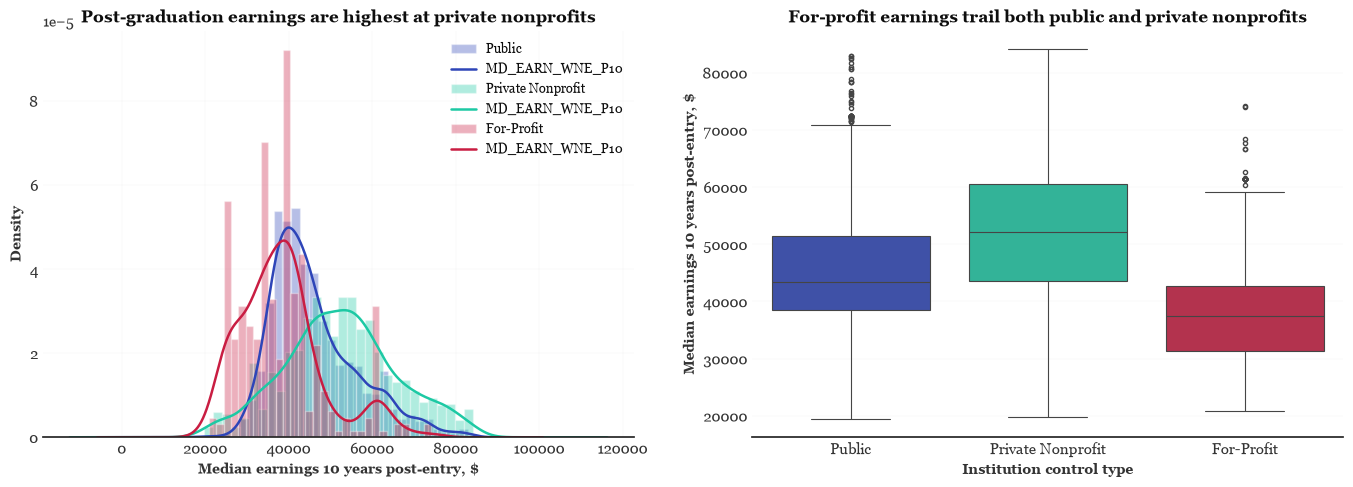
\includegraphics[width=\textwidth]{figures/figure1_earnings_distribution.png}
\caption{Distribution of median post-graduation earnings by institutional sector. Left panel shows kernel density estimates. Right panel shows boxplots. Private nonprofit graduates show the highest but most variable earnings. For-profit graduates are concentrated at the lowest levels.}
\label{fig:earnings_dist}
\end{figure}

\subsubsection{Question 2: How does tuition vary by sector?}

Tuition distributions are more sharply separated than earnings distributions. Figure~\ref{fig:tuition_violin} reveals three distinct pricing regimes. Public institutions charge a median of \$5,981, and fewer than 10\% exceed the national median of \$12,221. Private nonprofits charge a median of \$33,928, nearly three times the national median, with 91.2\% of institutions pricing above it. For-profit institutions charge a median of \$16,326, which falls halfway between the public and nonprofit levels, yet 84.4\% still charge above the national median. The contrast with the earnings distribution is stark: public institutions produce competitive earnings from roughly one-fifth the tuition base of private nonprofits.

\begin{figure}[htbp]
\centering
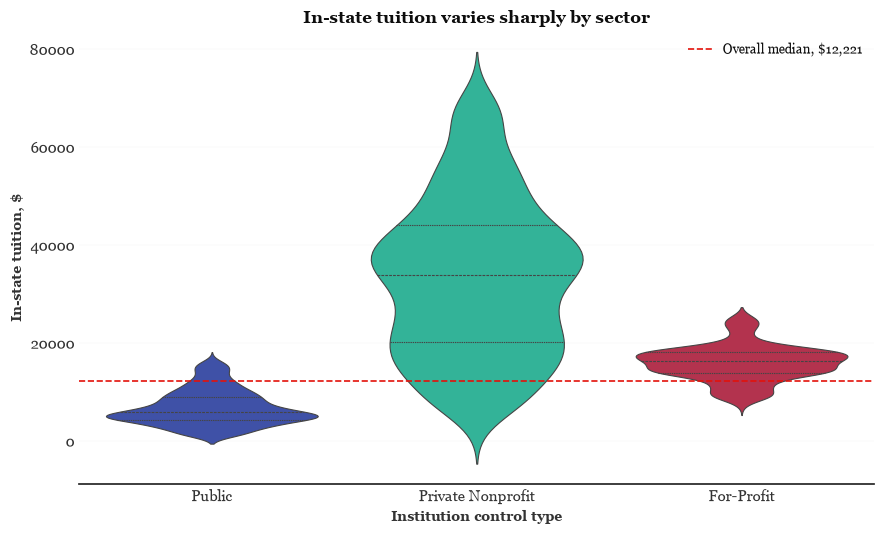
\includegraphics[width=\textwidth]{figures/figure6_tuition_violin.png}
\caption{In-state tuition distribution by sector with the national median (\$12,221) marked as a dashed red line. Public tuition is compressed in a low band. Private nonprofit tuition spans an extremely wide range. For-profit tuition is tightly clustered above the national median.}
\label{fig:tuition_violin}
\end{figure}

\subsubsection{Question 3: Do tuition and earnings form distinct clusters by sector?}

Figure~\ref{fig:tuition_earnings} presents the joint relationship. The three sectors form distinct clusters rather than a single continuum. Public institutions occupy a compact region of low tuition and moderate earnings. Private nonprofits stretch across a wide tuition range with highly variable earnings. For-profit institutions cluster in a narrow tuition band but show the lowest earnings conditional on tuition.

The overall Spearman rank correlation between tuition and earnings is 0.464 (p $<$ .001), confirming a statistically significant positive monotonic relationship. Stratified by sector, the correlations diverge considerably. Public institutions show the strongest association at 0.629. Private nonprofits follow at 0.587. For-profit institutions show a substantially weaker correlation of 0.335, indicating that tuition is a far less reliable signal of future earnings in that sector.

\begin{figure}[htbp]
\centering
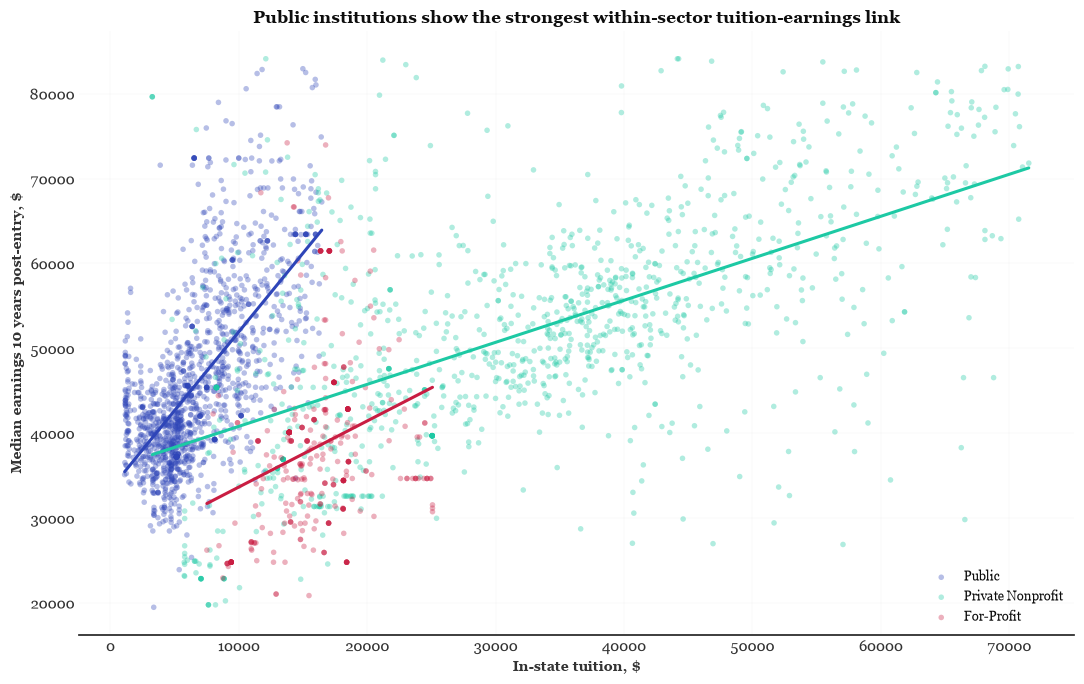
\includegraphics[width=\textwidth]{figures/figure2_tuition_earnings_scatter.png}
\caption{Tuition and earnings by institutional sector with linear regression lines. The three sectors form distinct clusters with different slopes and intercepts. The for-profit cloud sits below the other two at every tuition level.}
\label{fig:tuition_earnings}
\end{figure}

\subsubsection{Question 4: How does graduate debt relate to tuition and earnings?}

Graduate debt complicates the simple tuition-earnings story. Figure~\ref{fig:debt_mediation} shows two patterns. First, tuition and debt correlate positively in all three sectors. The correlation is strongest in the public sector (Spearman r = 0.729), reflecting a direct pass-through of costs to students. Private nonprofits show a ceiling effect where debt plateaus around \$25,000 despite tuition reaching \$80,000, consistent with federal borrowing limits constraining debt even at high tuition levels.

Second, the debt-to-earnings ratio reveals the real divide. Public graduates carry a median ratio of 0.29, roughly twenty-nine cents of debt for every dollar of annual earnings. Private nonprofit and for-profit graduates carry ratios of 0.45 and 0.43, respectively. The cost of financing education through debt erodes the net return, and it does so most severely outside the public sector. This finding adds weight to the research question: if students in different sectors face systematically different debt burdens, the net benefit of a tuition investment cannot be evaluated on earnings alone.

\begin{figure}[htbp]
\centering
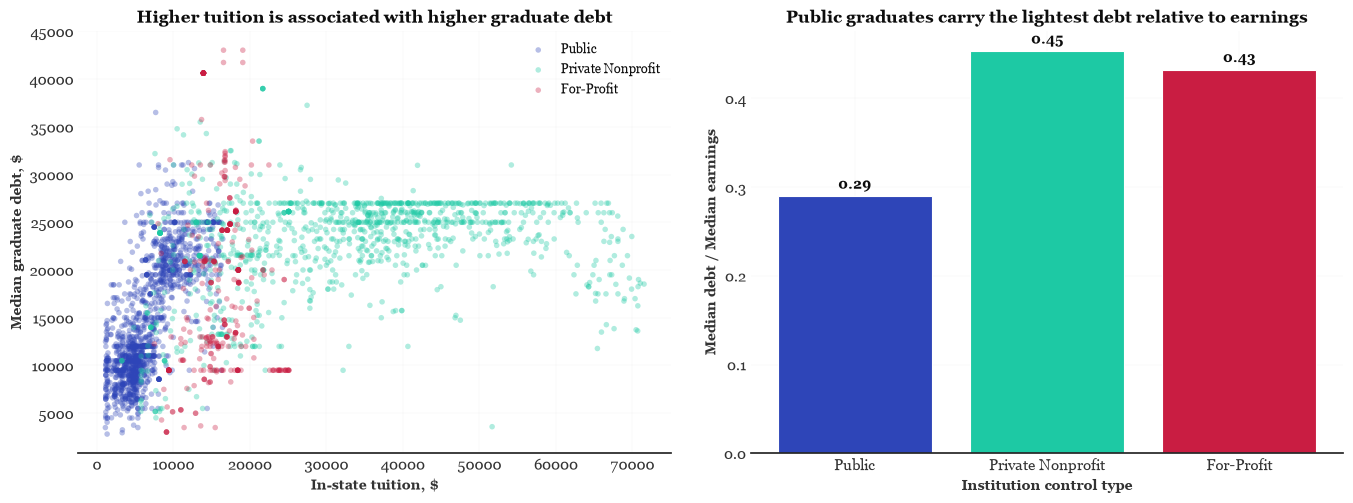
\includegraphics[width=\textwidth]{figures/figure7_debt_mediation.png}
\caption{Left panel: tuition versus graduate debt by sector. Right panel: median debt-to-earnings ratio by sector. Public graduates carry the lightest debt burden relative to their earnings.}
\label{fig:debt_mediation}
\end{figure}

\subsubsection{Question 5: Does selectivity explain the tuition-earnings link?}

Admission rate data are available for roughly half the sample, so this question is examined as a stratified analysis rather than a control variable. Figure~\ref{fig:selectivity} shows a clear selectivity gradient: more selective institutions produce higher earnings in every sector. Among highly selective institutions, private nonprofit graduates earn a median of \$63,952 compared to \$54,064 in the less selective tier.

The tuition-earnings correlation persists within selectivity tiers for public and private nonprofit institutions. Public institutions maintain a significant Spearman correlation of 0.404 within the reporting subset, and private nonprofits show a correlation of 0.551. The for-profit sector produces a negative but unreliable estimate in this restricted sample, driven by the small number of for-profit institutions that report admission rates. Selectivity therefore explains part of the earnings variation but does not eliminate the sector-level pattern.

\begin{figure}[htbp]
\centering
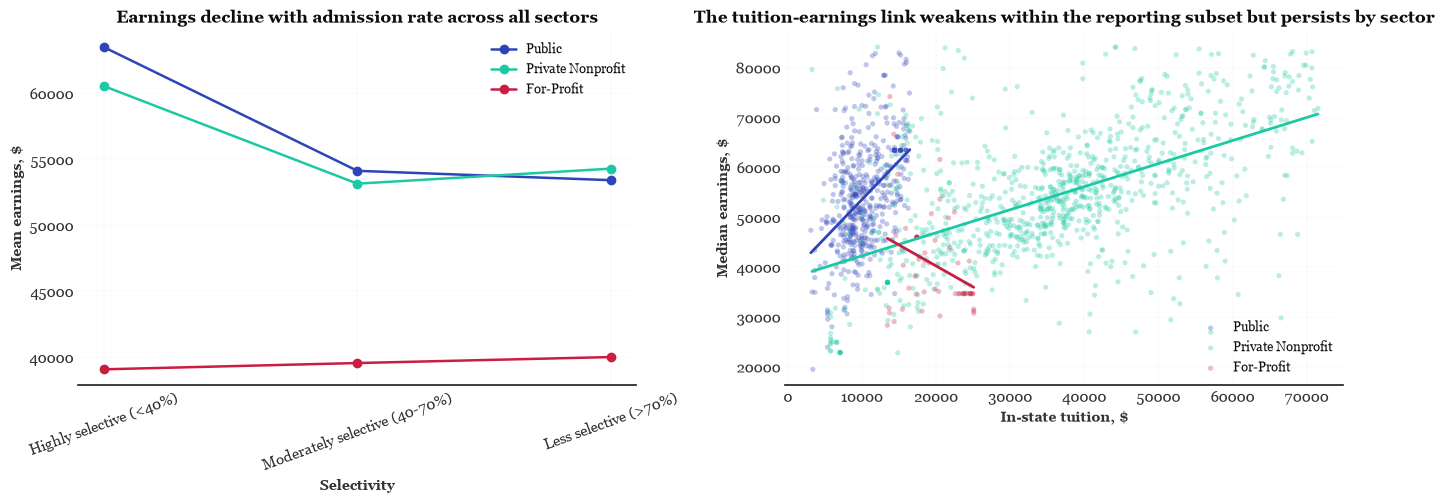
\includegraphics[width=\textwidth]{figures/figure8_selectivity_analysis.png}
\caption{Left panel: mean earnings by selectivity tier and sector. Right panel: tuition-earnings scatter within the admission-reporting subset with regression lines. The sector gradient persists after accounting for selectivity.}
\label{fig:selectivity}
\end{figure}

\subsubsection{Question 6: Do minority-serving institutions differ from non-MSIs?}

Minority-serving institutions operate on a structurally different cost-outcome curve within every sector. Figure~\ref{fig:msi} shows that MSIs charge lower median tuition and report lower median earnings than their non-MSI counterparts. The gap is most visible in the public sector, where MSIs charge a median of \$5,193 against \$6,361 for non-MSIs, and their graduates earn a median of \$43,172 against \$44,298.

Public MSIs also generate lower median graduate debt (\$11,631 versus \$13,532). These institutions succeed in minimizing front-end costs and debt burdens. The persistently lower earnings, however, point to an equity dimension: these institutions serve populations that face broader socioeconomic and labor market barriers that the tuition-earnings models cannot capture. This finding does not directly test the research question, but it adds context: if the tuition-earnings relationship differs by sector, and MSIs within each sector sit at the lower end of both distributions, the net return equation is not uniform even within sectors.

\begin{figure}[htbp]
\centering
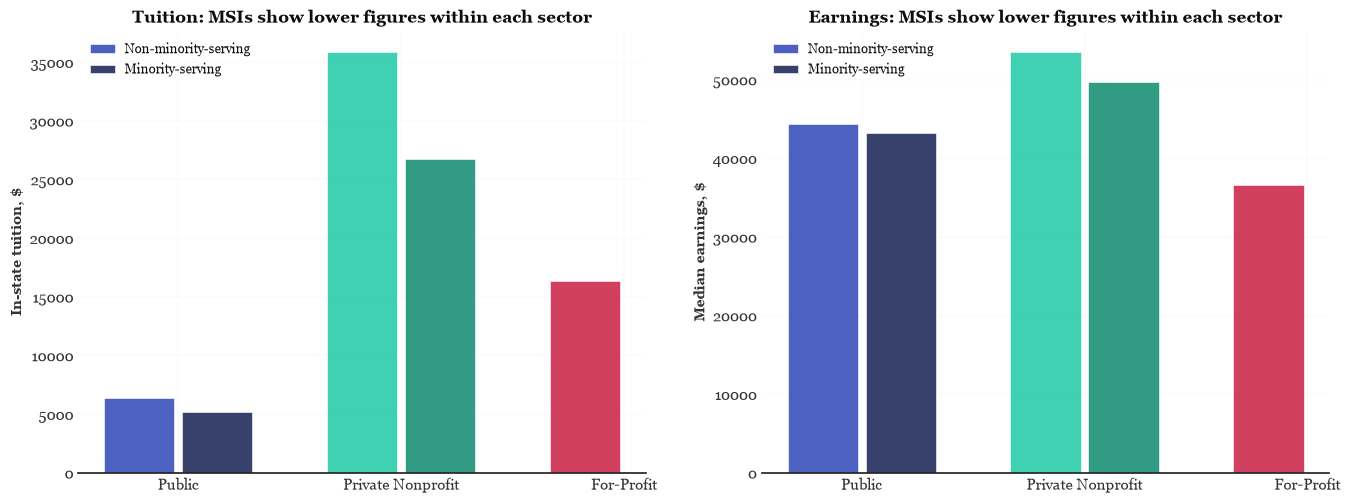
\includegraphics[width=\textwidth]{figures/figure9_msi_comparison.png}
\caption{Median tuition and median earnings by sector, comparing minority-serving institutions against non-minority-serving institutions. MSIs charge less and their graduates earn less within every sector.}
\label{fig:msi}
\end{figure}

\subsection{Preliminary Inference}

Before estimating the regression models, the earnings distribution was tested for normality. The D'Agostino K-squared test confirmed that the distribution deviates significantly from a Gaussian curve (p $<$ .001). With nearly 3,000 observations, the test is sensitive enough to detect even trivial departures from normality. The visual diagnostics in Figure~\ref{fig:normality} provide a more practical assessment. The histogram reveals a mixture distribution: the primary mode near \$42,000 is driven by the dense public sector, the right shoulder near \$60,000 reflects the elite private nonprofit tier, and the left tail near \$20,000 captures for-profit institutions. The Q-Q plot confirms that the data are approximately normal in the central interquartile range but exhibit lighter tails at both extremes.

\begin{figure}[htbp]
\centering
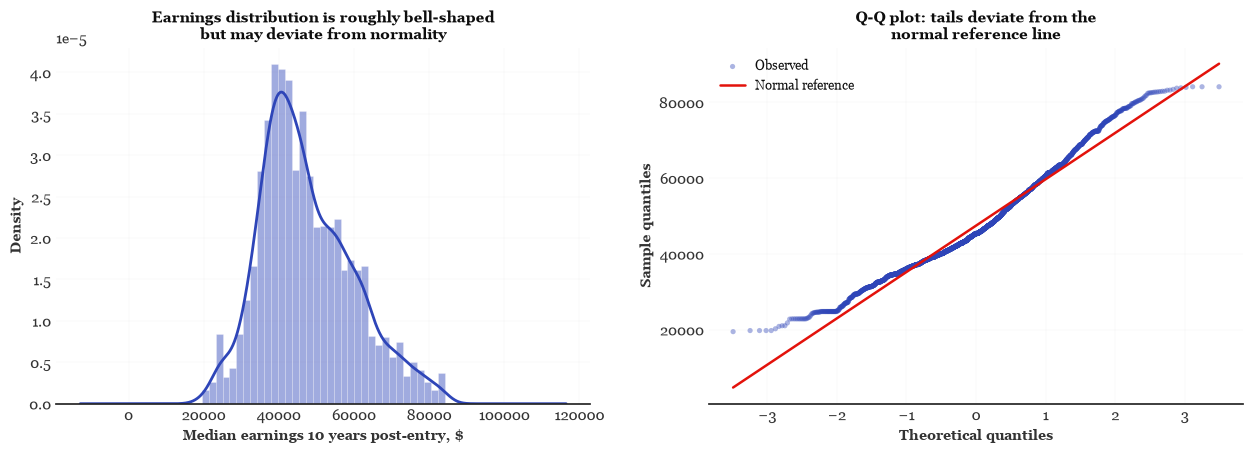
\includegraphics[width=\textwidth]{figures/figure10_normality_diagnostics.png}
\caption{Left panel: histogram of median earnings with kernel density estimate. Right panel: Q-Q plot against the normal distribution. The distribution shows a mixture of three sector-level components and lighter tails than a normal curve.}
\label{fig:normality}
\end{figure}

The non-normal and heteroskedastic structure of the data supports the use of Spearman's rank correlation for the preliminary association test. The global Spearman correlation between in-state tuition and median earnings is 0.464 (p $<$ .001), explaining roughly 21.5\% of the variance in earnings ranks. This confirms that a significant positive relationship exists at the aggregate level. But as the exploratory figures demonstrate, this global estimate is a weighted average of three sector-specific slopes that differ in both magnitude and reliability.

\subsection{Regression Results}

The three models form a nested sequence. Model 1 estimates the pooled association. Model 2 adds sector interactions. Model 3 tests whether the sector differences persist after adjusting for enrollment, degree level, and state fixed effects. Table~\ref{tab:model_fit} compares the fit statistics across all three models.

\begin{table}[htbp]
\centering
\caption{Model Fit Comparison}
\label{tab:model_fit}
\begin{tabular}{lcccccc}
\toprule
\textbf{Model} & \textbf{N} & \textbf{R$^2$} & \textbf{Adj. R$^2$} & \textbf{Log RMSE} & \textbf{AIC} & \textbf{BIC} \\
\midrule
Model 1 & 2,894 & 0.187 & 0.187 & 0.236 & $-$153.0 & $-$141.1 \\
Model 2 & 2,894 & 0.398 & 0.397 & 0.203 & $-$1,013.5 & $-$977.7 \\
Model 3 & 2,894 & 0.591 & 0.582 & 0.178 & $-$2,383.1 & $-$2,159.9 \\
\bottomrule
\end{tabular}
\vspace{6pt}
{\footnotesize \textit{Note.} Log RMSE is the root mean squared error of the log-transformed residuals. All models use HC3 standard errors.}
\end{table}

\subsubsection{Model 1: Unconditional Association}

Model 1 estimates a pooled tuition elasticity of 0.121 across all 2,894 institutions, with a 95\% confidence interval of [0.113, 0.129] and p $<$ .001. The model explains 18.7\% of the variation in log earnings. The Breusch-Pagan test rejects homoskedasticity (p $<$ .001), confirming the need for HC3 standard errors.

Translating to practical terms, a student comparing a \$6,000 public tuition against a \$34,000 private nonprofit tuition would face roughly a fivefold difference. The model predicts about a 0.9\% earnings advantage for the higher-tuition institution, or roughly \$400 on a \$45,000 median starting salary. The relationship is statistically reliable but economically modest. The residual diagnostics in Figure~\ref{fig:model1_diagnostics} show heavier tails than a normal distribution and widening residual spread at higher fitted values, confirming that the pooled model fits poorly across the range of the data.

\begin{figure}[htbp]
\centering
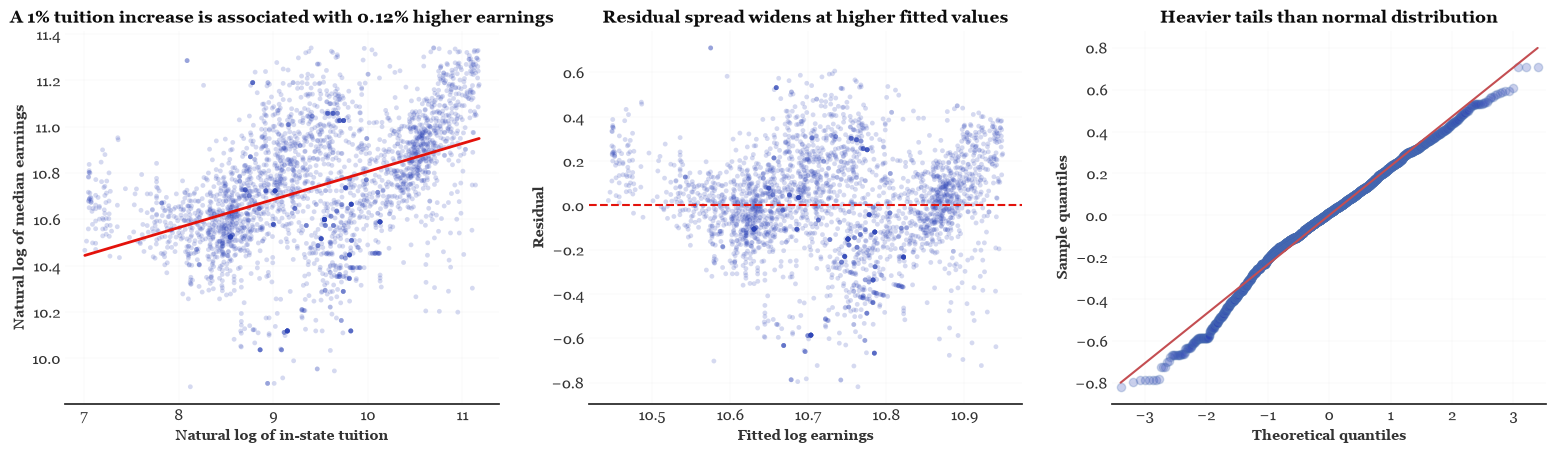
\includegraphics[width=\textwidth]{figures/figure3_model1_diagnostics.png}
\caption{Model 1 diagnostics. Left panel: log-log scatter with the pooled regression line. Center panel: residuals against fitted values, showing heteroskedasticity. Right panel: Q-Q plot of residuals with heavier tails than a normal distribution.}
\label{fig:model1_diagnostics}
\end{figure}

This pooled estimate addresses the first part of the research question. A significant positive relationship exists between tuition and earnings. But the exploratory analysis has already shown that the three sectors operate on different cost-outcome curves, and the residual diagnostics confirm that a single slope cannot represent them accurately. The second part of the research question requires the sector interaction model.

\subsubsection{Model 2: Sector Interaction}

Adding sector indicators and tuition-by-sector interactions raises the adjusted R-squared from 0.187 to 0.397. The log RMSE drops from 0.236 to 0.203. The AIC falls from $-$153 to $-$1,013. Accounting for sector more than doubles the explained variance.

The estimated tuition elasticities are 0.194 for public institutions (95\% CI [0.176, 0.213]), 0.277 for private nonprofits (95\% CI [0.242, 0.312]), and 0.400 for for-profits (95\% CI [0.301, 0.499]). Each slope is positive with p $<$ .001. The joint Wald test for the interaction terms yields a statistic of 30.122 with p $<$ .001, confirming that the tuition-earnings slope differs across sectors. This directly answers the second part of the research question: the relationship is not uniform.

The range is practically meaningful. A student comparing identical tuition levels would expect roughly twice the earnings increment at a for-profit institution compared to a public institution. Figure~\ref{fig:sector_scatter} shows the fitted lines in log-log space. The for-profit line is the steepest, but it operates in a region of the data where for-profit institutions are concentrated in particular states, offer predominantly sub-baccalaureate credentials, and enroll smaller student bodies. Their high apparent elasticity is a composition effect, not a genuine sector advantage.

\begin{figure}[htbp]
\centering
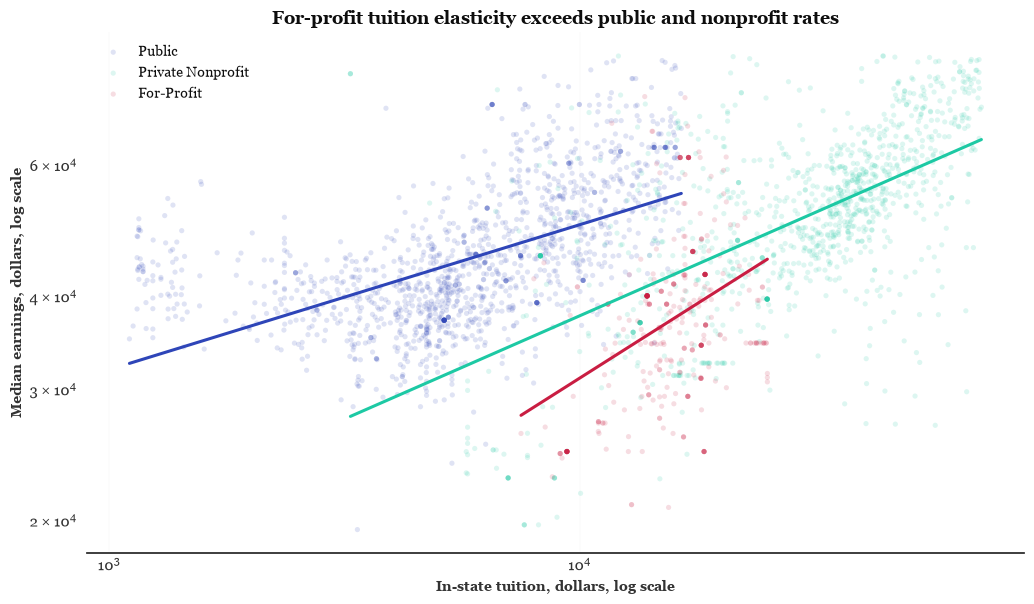
\includegraphics[width=\textwidth]{figures/figure4_sector_loglog.png}
\caption{Log-log scatter of tuition and earnings by sector with Model 2 fitted lines. The for-profit line is the steepest but reflects composition rather than a genuine sector advantage. Public and nonprofit lines show more moderate slopes.}
\label{fig:sector_scatter}
\end{figure}

\subsubsection{Model 3: Institutional-Control Robustness}

Model 3 adds undergraduate enrollment, predominant degree, and state fixed effects to the Model 2 specification. The adjusted R-squared rises to 0.582, and the log RMSE falls to 0.178. The added controls are jointly significant with Wald p $<$ 10$^{-265}$, confirming that institutional characteristics beyond tuition explain a substantial share of earnings variation.

After adjustment, the tuition elasticities converge to a narrow range. Table~\ref{tab:elasticities} reports the estimates and confidence intervals for Models 2 and 3.

\begin{table}[htbp]
\centering
\caption{Sector-Specific Tuition Elasticities with 95\% Confidence Intervals}
\label{tab:elasticities}
\begin{tabular}{lcccc}
\toprule
 & \multicolumn{2}{c}{\textbf{Model 2}} & \multicolumn{2}{c}{\textbf{Model 3}} \\
\textbf{Sector} & \textbf{Elasticity} & \textbf{95\% CI} & \textbf{Elasticity} & \textbf{95\% CI} \\
\midrule
Public & 0.194 & [0.176, 0.213] & 0.189 & [0.168, 0.210] \\
Private Nonprofit & 0.277 & [0.242, 0.312] & 0.147 & [0.116, 0.178] \\
For-Profit & 0.400 & [0.301, 0.499] & 0.119 & [0.034, 0.205] \\
\bottomrule
\end{tabular}
\vspace{6pt}
{\footnotesize \textit{Note.} All elasticities are from log-log OLS models with HC3 standard errors. Model 3 includes controls for log enrollment, categorical degree level with bachelor's as reference, and state fixed effects.}
\end{table}

The central result is the collapse of the for-profit elasticity from 0.400 to 0.119, a reduction of roughly 70\%. The private nonprofit estimate falls from 0.277 to 0.147. The public estimate remains essentially unchanged at 0.189. Figure~\ref{fig:coef_plot} visualizes this shift.

\begin{figure}[htbp]
\centering
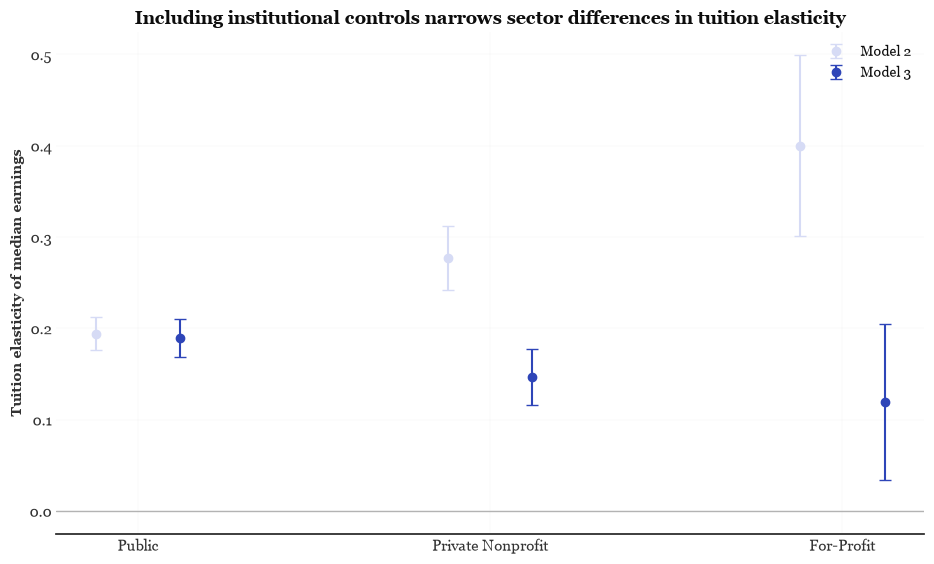
\includegraphics[width=\textwidth]{figures/figure5_coefficient_plot.png}
\caption{Tuition elasticity estimates by sector for Model 2 (unadjusted) and Model 3 (with controls). Error bars show 95\% confidence intervals. The sector differences narrow substantially after adding institutional controls.}
\label{fig:coef_plot}
\end{figure}

The joint tuition-by-sector interaction test yields p = 0.047 in Model 3, falling just below the conventional 0.05 threshold. The remaining sector differences, while statistically detectable, are narrow in practical terms. The three elasticities span a range of 0.07 percentage points. For a student facing a \$10,000 tuition difference between two institutions, the predicted annual earnings gap is \$189 at a public institution, \$147 at a nonprofit, and \$119 at a for-profit. Whether a range of \$70 in predicted annual earnings across sectors constitutes a meaningful policy difference is a judgment the data cannot make.

The controls themselves explain roughly 19 additional percentage points of earnings variance beyond Model 2. Institutional location, size, and degree mix matter more for earnings than the tuition price. This finding reframes the research question: the answer is that the relationship exists and differs by sector, but the differences are substantially smaller than the unadjusted estimates suggest, and the practical magnitude of those differences is modest.

\subsection{Sensitivity Analysis: Admission Rate}

Admission rate data are available for only 1,466 of the 2,894 institutions. The reporting subset overrepresents private nonprofits (908 institutions) and underrepresents for-profits (55 institutions). Two models estimated on this restricted sample test whether adding selectivity changes the main results.

Within the reporting subset, the Model 3 specification without admission rate produces tuition elasticities comparable to the full-sample estimates for public and nonprofit institutions. Adding admission rate leaves those elasticities positive and significant: 0.175 for public institutions (p $<$ .001) and 0.128 for private nonprofits (p $<$ .001). The for-profit estimate becomes negative at $-$0.044 with p = 0.823 and a wide confidence interval. Admission rate itself has a coefficient of $-$0.103 (p $<$ .001), indicating that more selective institutions produce higher earnings conditional on the other controls.

The sector interactions are not jointly significant in the restricted model (p = 0.155). The sensitivity analysis therefore supports the main tuition result for public and private nonprofit institutions but cannot validate it for the for-profit subset. Missing admission rates are unlikely to be random, because selective institutions are disproportionately likely to report their rates. The restricted estimates must not be generalized to all institutions.

\subsection{Answering the Research Question}

The research question asked two things. First, is there a significant relationship between in-state tuition and median post-graduation earnings? The answer is yes. Every model finds a positive and statistically significant association in every sector, before and after adjustment. Second, does this relationship differ across public, private nonprofit, and for-profit institutions? The answer is yes, but with an important qualification. The unadjusted sector differences are large: for-profit elasticities appear to be roughly double the public estimate in Model 2. Once enrollment, degree level, and state fixed effects are held constant, those differences narrow to a range of 0.07 elasticity points. The sector interaction remains marginally significant at p = 0.047, but the economic magnitude of the remaining gap is small.

The practical implication is that the tuition-earnings relationship is real but not a straightforward guide for decision-making. Students choosing between institutions will find more signal in the sector itself, the state where the institution is located, and the type of degree offered than in the tuition price alone. For policymakers, the narrow range of elasticities across sectors after adjustment suggests that regulatory attention to tuition pricing may be less productive than attention to the structural characteristics that predict earnings independent of price.
